\documentclass[12pt]{article}
\usepackage{graphicx}
\usepackage{float}
\usepackage{titling}

\setlength{\droptitle}{-10em}

\title{Temperature Autocorrelation in Key West}
\author{Sam Turner}
\date{}
\begin{document}
    \maketitle
    \begin{abstract}
    Temporal autocorrelation is found in temperatures recorded in Key West between 1901 and 2000.

    \end{abstract}


    \section{Introduction}
        When interpreting any data set, it is important to consider the process which generates the data. In the case of a time series, values may be correlated with earlier values, meaning that successive measurements are not independant. Here, we check for lag-1 autocorrelation in Key West temperature data:

        \begin{figure}[H]
        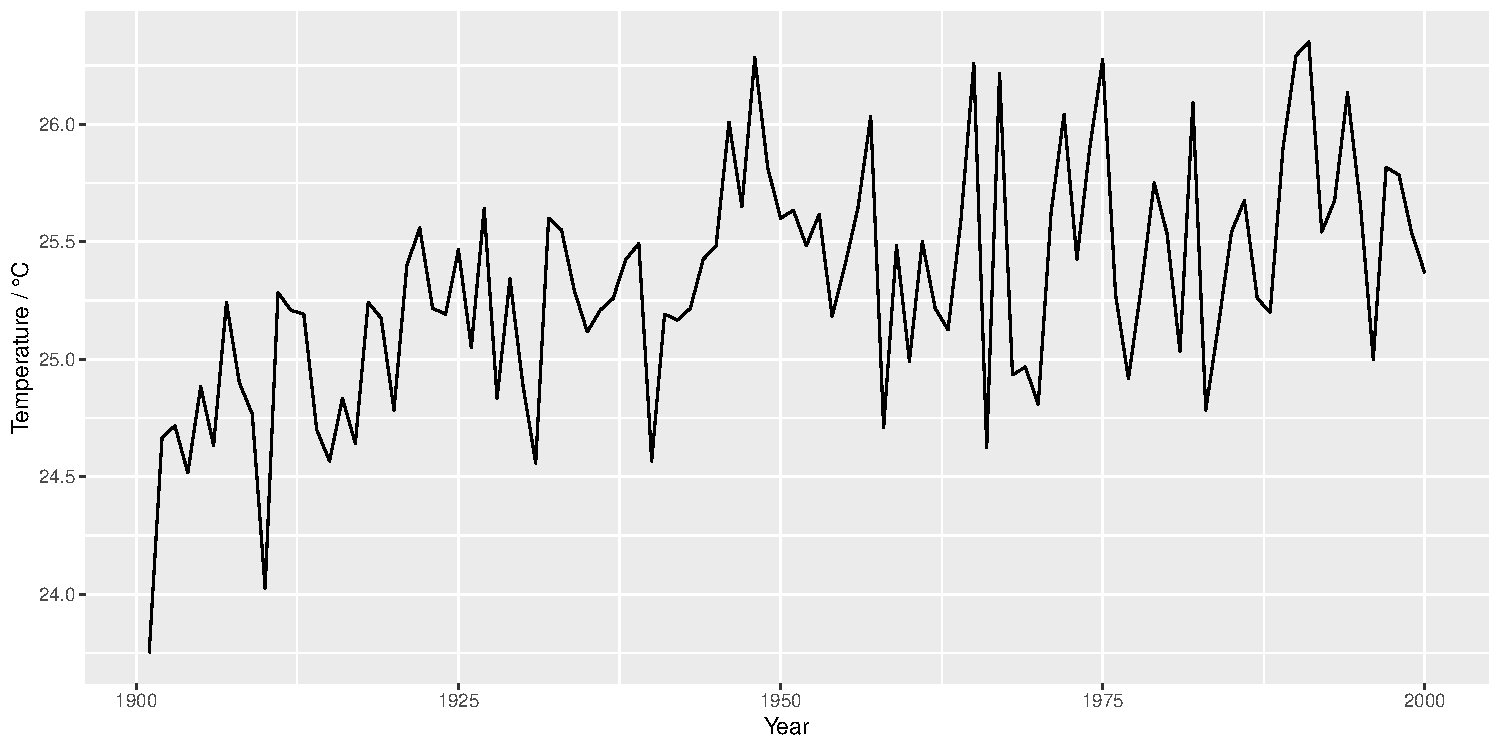
\includegraphics[width=\linewidth]{../Results/TempTimeSeries.pdf}
        \caption{Time series of Key West Temperatures}
        \label{fig:temptimeseries}
        \end{figure}
        

    \section{Materials and Methods}


        We determined the correlation coefficient between a 99-length vector containing yearly temperatures between 1901 and 1999 ($x_{t0}$), and the vector containing temperatures from 1902 and 2000 ($x_{t1}$). This correlation coefficient was compared to the correlation coefficient between similarly offset 99-length vectors obtained by discarding either the  first or last value from 100,000 random permutations of the Key West temperatures. The proportion of these values which are equal to or higher than the true correlation coeeficient gives an approximation of the probability of seeing the observed level of yearly correlation given the measurements observed and is therefore our approximate p-value. 



    \section{Results}

        We find a correlation coefficient of 0.3261697 between $x_{t0}$ and $x_{t1}$. The proportion of scrambled data correlation coefficients (our aproximate p value) which are greater than this is 0.0004:

        \begin{figure}[H]
        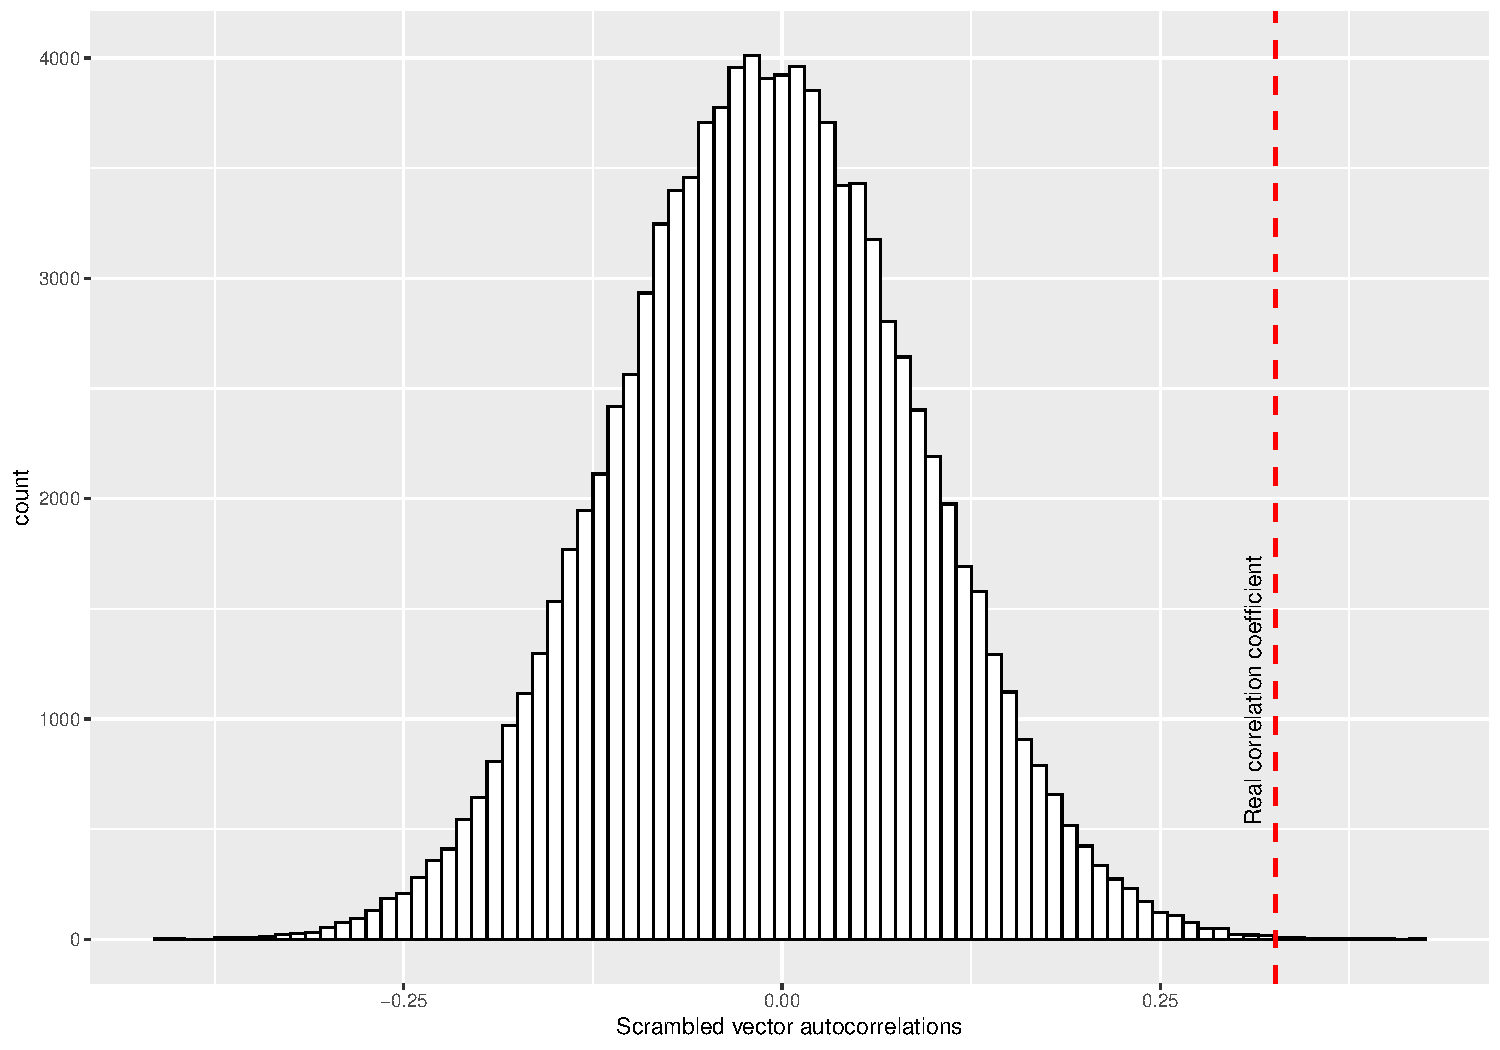
\includegraphics[width=\linewidth]{../Results/AutoC.pdf}
        \caption{Distribution of correlation coefficients for randomly permuted temperature vectors}
        \label{fig:corrcoef}
        \end{figure}

        \pagebreak
        \noindent
        Indeed, when we look at a scatter of $x_{t}$ against $x_{t+1}$, there appears to be a positive correlation. 


        \begin{figure}[H]
        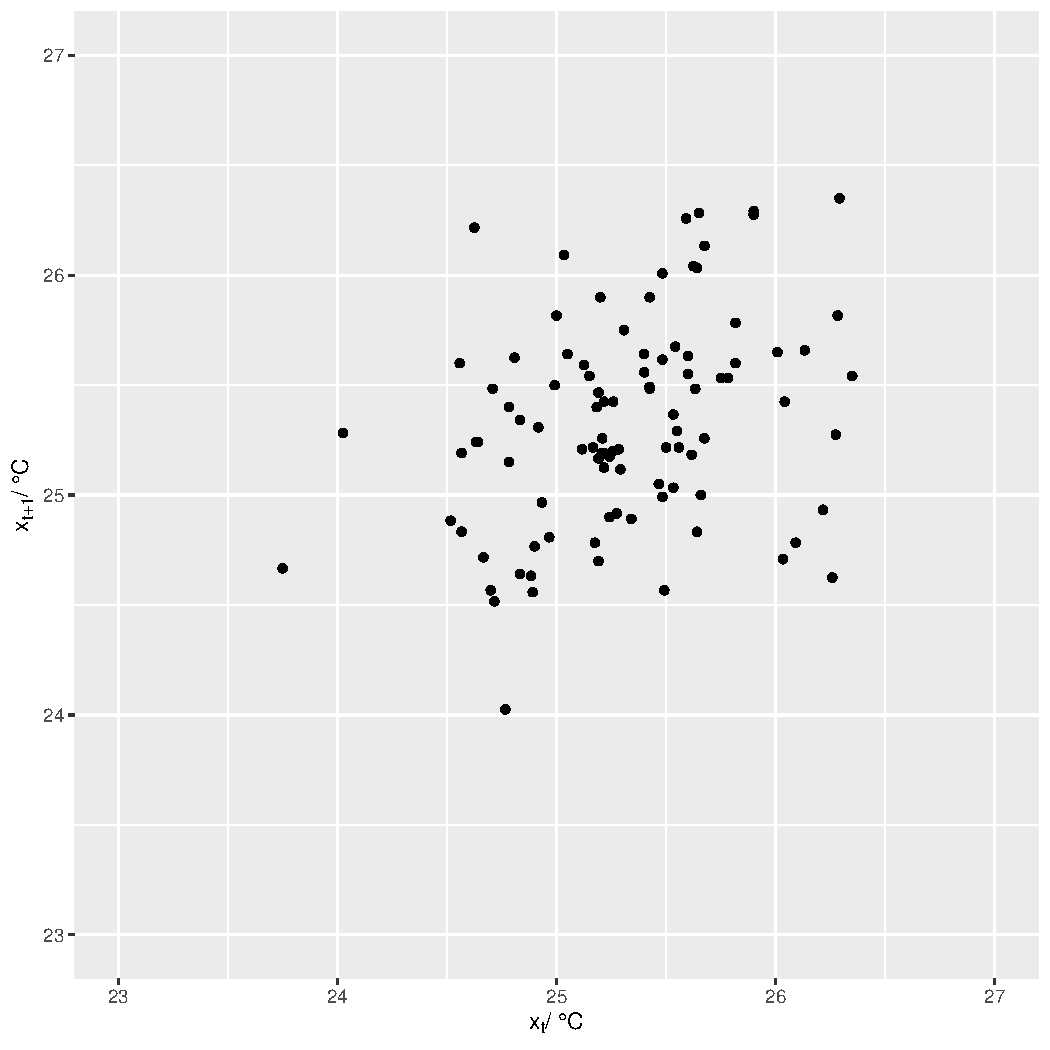
\includegraphics[width=\linewidth]{../Results/AutoCscatter.pdf}
        \caption{Scatter of $x_{t}$ against $x_{t+1}$}
        \label{fig:scatter}
        \end{figure}

\end{document}
